
%%%%%%%%%%%%%%%%%%%%%
\section{Champ de température}
%%%%%%%%%%%%%%%%%%%%%
%
La donnée de la température en tout point de l'espace-temps permet de définir le "champ de température". Ce champ peut être mesuré en un lieu et à une date particulière à l'aide d'un thermomètre.
Le graphe suivant représente le champ de température moyenne sur la surface de la terre, ce champ ne dépend pas du temps

\begin{center}
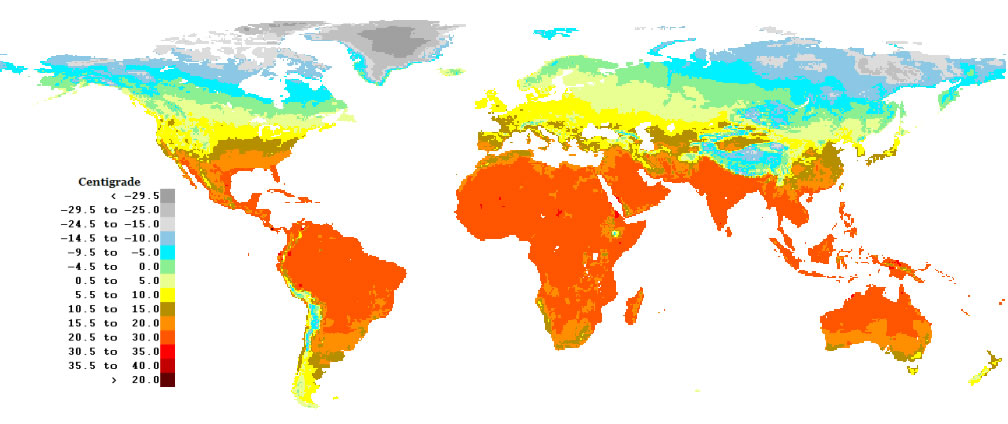
\includegraphics[scale=.45]{./champs/temperatures}
\end{center}



Ce champ de température moyenne est une application ($\Theta_M$) qui associe une température ($\theta_M$) à chaque point ($x,y$) de la surface de la terre.

\begin{align*}
\Theta_M :\ \ \ \ \ \ \ \ \mathbb{R} ^2 \ \  & \rightarrow \ \ \mathbb{R} \\
(x,y) \ \ & \mapsto \ \ \theta_M = \Theta_M(x,y)
\end{align*}

La température dépend du temps (de la date) et des trois dimensions de l'espace,
le champ de température ($\Theta$) est donc une application qui associe une température ($\theta$) à chaque point ($x,y,z,t$) de l'espace-temps.

\begin{align*}
\Theta :\ \ \ \ \ \ \ \ \ \ \ \ \mathbb{R} ^4 \ \  & \rightarrow \ \ \mathbb{R} \\
(x,y,z,t) \ \ & \mapsto \ \ \theta = \Theta(x,y,z,t)
\end{align*}



%%%%%%%%%%%%%%%%%%%%%%%%%%%%%%%%%%%%%%%%%%%%%%%%%%%%%%%%%%%%%%%%%%%%%%%%%%%%
